
\chapter{Espacios vectoriales $\divideontimes$}	\label{e_vec}

La idea de vector está tomada de la Física, donde sirven para representar magnitudes vectoriales como fuerzas, velocidades o aceleraciones. Para ello se emplean vectores de dos componentes en el plano, de tres componentes en el espacio... 

En Matemáticas, se trata de abstraer las propiedades que caracterizan a los vectores para extenderlas también a otro tipo de objetos diferentes de los vectores de la Física. Esencialmente, el comportamiento que caracteriza a los vectores es el siguiente: 

\hspace{3mm} * Podemos sumar dos vectores y obtenemos otro vector; 

\hspace{3mm} * Podemos multiplicar un vector por un número (escalar) y obtenemos otro vector. 

En álgebra abstracta, un espacio vectorial (o también llamado espacio lineal) es una estructura algebraica creada a partir de un conjunto no vacío, una operación interna (llamada suma, definida para los elementos del conjunto) y una operación externa (llamada producto por un escalar, definida entre dicho conjunto y otro conjunto, con estructura de  cuerpo), con unas propiedades fundamentales.

A los elementos de un espacio vectorial se les llama vectores ($\vec u, \vec v, \vec w, \cdots  $)y a los elementos del cuerpo, escalares ($\alpha, \beta, \gamma, \cdots$).

\section{Espacios vectoriales}

\begin{defi} Se llama `espacio vectorial' $\mathcal V$ sobre un cuerpo $\mathcal K$ a la terna : $\; \; $ \colorbox{LightYellow}{$\displaystyle \left( \; (\mathcal V, \oplus),\; (\mathcal K,+,\cdot),\; \odot \;  \right) $} $\quad$, donde $(\mathcal V, \oplus)$ es un grupo abeliano a cuyos elementos se les llama vectores ($\vec u, \vec v, \vec w, \cdots  $), $(\mathcal K, +, \cdot)$ es un cuerpo conmutativo a cuyos elementos se les llama escalares ($\alpha, \beta, \gamma, \cdots$) y $\odot$ es una ley de composición externa de $\mathcal K$ sobre $\mathcal V$, de modo que $\forall \alpha \in \mathcal K \; \wedge \; \forall \vec u \in \mathcal V \rightsquigarrow \alpha \odot \vec u \in \mathcal V$ , donde se han de cumplir cuatro propiedades:

\begin{enumerate}[EV.1. ]

\item $\lambda \odot (\vec u \oplus \vec v)= (\lambda \odot \vec u) \; \oplus \; (\lambda \odot \vec v)$
\item $(\lambda + \mu)\odot \vec u = (\lambda \odot \vec u) \; \oplus \; (\mu \odot \vec u)$
\item  $(\lambda \cdot \mu)\odot \vec u = \lambda \odot (\mu \odot \vec u)$
\item $1\odot \vec v = \vec v$
$\qquad \qquad \qquad \qquad \forall \lambda, \mu \in \mathcal K; \; \; \forall \vec u, \vec v \in \mathcal V$	
\end{enumerate}
\end{defi}

En adelante usaremos los mismos símbolos para la suma de vectores que de escalares, así como para el producto de escalares y el de un escalar por un vector: $\lambda + \mu; \quad \vec u + \vec v; \quad \lambda \cdot \mu; \quad \lambda \cdot \vec u$ o, simplemente $\lambda \mu; \quad \lambda \cdot \vec u$ o, simplemente $\lambda \vec u$ y también en adelante $\mathcal K \equiv \mathbb R$ y hablaremos de \colorbox{LightYellow}{`espacios vectoriales reales'}, que representaremos más sencillamente por \colorbox{LightYellow}{$(\mathcal V, +, \cdot)$},  donde $+$ es la ley de composición interna en $\mathcal V$, la suma de vectores y $\cdot$  es la ley de composición externa de $\mathbb R$ sobre $\mathcal V$, el producto de un número real (escalar) por un vector.

\begin{ejem}.

\begin{itemize}

\item $\mathbb R; \; \mathbb R^2; \; \mathbb R^3$ y, en general $\mathbb R^n$  son espacios vectoriales reales con las operaciones usuales de ley suma de vectores y producto por un escalar:

$(u_1,u_2,u_3, \cdots, u_n)\; +\; (v_1,v_2,v_3, \cdots v_n)=(u_1+v_1, u_2+v_2, u_3+v_3, \cdots , u_n+v_n)$

 $\alpha \cdot (u_1,u_2,u_3, \cdots, u_n) =(\alpha u_1,\alpha u_2,\alpha u_3, \cdots, \alpha u_n)$

\item $(\mathcal M_{m \times n}(\mathbb R),+,\cdot)$ es el espacio vectorial de las matrices reales de orden $m \times n$ con las operaciones aprendidas en el tema de matrices.

\item $(\mathcal P_n(\mathbb R), +, \cdot)$ es el espacio vectorial de los polinomios de una variable real de grado menor o igual a $n$ con las operaciones habituales de suma de polinomios y producto de un polinomio por un número real.

\item $(\mathcal C_0(\mathbb R), +, \cdot)$ es el espacio vectorial de las funciones reales de variable real `continuas' con las operaciones habituales de suma y producto por un número.
\end{itemize}
\end{ejem}

\begin{prop} Sea $\mathcal V$ un e.v. real, entonces:
\begin{enumerate}[P1. ]
\item $\alpha \; \vec 0=\vec 0,\quad \forall \alpha \in \mathbb R$
\item $0 \; \vec u= \vec 0, \quad \forall \vec u \in \mathcal V$
\item $\alpha \; \vec u = \vec 0 \leftrightarrow \alpha = 0 \; \vee \; \vec u= \vec 0, \quad \forall \alpha \in \mathbb R,\; \forall \vec u \in \mathcal V$
\item $(-\alpha)\; \vec u=-(\alpha \; \vec u)=\alpha\;  (-\vec u),  \quad \forall \alpha \in \mathbb R,\; \forall \vec u \in \mathcal V$
\item $\alpha \; \vec u = \alpha\; \vec v \; \wedge \; \alpha \neq 0 \to \vec u = \vec v, \quad \forall \alpha \in \mathbb R,\; \forall \vec u, \vec v \in \mathcal V$
\item $\alpha \; \vec u = \beta \; \vec u \; \wedge \, \vec u \neq \vec 0 \to \alpha = \beta, \quad \forall \alpha, \beta \in \mathbb R,\; \forall \vec u \in \mathcal V$
\item $(-\alpha)\; (-\vec u)= \alpha \; \vec u , \quad \forall \alpha \in \mathbb R,\; \forall \vec u \in \mathcal V$
	
\end{enumerate}	
\end{prop}


\subsection{Subsespacio vectorial}

\begin{defi}
Sea $\mathcal V$ un espacio vectorial y sea $\mathcal W \subset \mathcal V$ un subconjunto de $\mathcal V$. Decimos que $\mathcal W$ es un `subespacio vectorial de $\mathcal V$' si:

\vspace{2mm}
\centerline{\colorbox{LightYellow}{$\boxed{\; \forall \vec u, \vec v \in \mathcal W \; \wedge \; \forall \lambda, \beta \in \mathbb R \quad \therefore \quad \lambda \vec u + \beta \vec v \in \mathcal W\; }$}}

\end{defi}

\justify

\begin{ejem}
Hay dos subespacios triviales en $\mathcal V$, el mismo 	$\mathcal V$ y $\{\vec 0\}$, se llaman subespacios impropios.

Ejemplos de subespacios vectoriales propios son:

\begin{itemize}
\item $\mathcal V = \mathbb R^2 \to \mathcal W_1= \{\vec 0\} \times \mathbb R; \quad \mathcal W_2= \mathbb R \times \{\vec 0\}$ son subespacios de $\mathbb R^2$

\textcolor{gris}{ \footnotesize{$\alpha (0,x) + \beta (0,y)=(0,\alpha x + \beta y) \in \mathcal W_1 ; \quad 
\alpha (x,0) + \beta (y,0)=(\alpha x + \beta y,0) \in \mathcal W_2 $}}

\item $\mathcal W=\{ (x,0,0) / x \in \mathbb R \} \subset \mathbb R^3$ es s.e.v. de $\mathbb R^3$.
\item $\mathcal W=\{ (x,y,0,t) / x,y,t \in \mathbb R \} \subset \mathbb R^4$ es s.e.v. de $\mathbb R^4$.
\item $\mathcal W=\{ M\in \mathcal M_{n \times n}(\mathbb R) \; / \; A^T=A\}$ es un s.e.v. de $\mathcal M_{n \times n}(\mathbb R)$
\item $\mathcal W=\{ M\in \mathcal M_{2 \times 2}(\mathbb R) \; / \; det(A)=0\}$ NO es un s.e.v. de $\mathcal M_{2 \times 2}(\mathbb R)$

\vspace{2mm} \textcolor{gris}{\small{ya que, p.e., las matrices: 
$A_1=\left( \begin{matrix} 1&0\\0&0 \end{matrix} \right); \quad 
A_2=\left( \begin{matrix} 0&0\\0&1 \end{matrix} \right) \; \in \mathcal W$,}}
 
\textcolor{gris}{ \small{pues $det(A_1)=det(A_2)=0\quad $, pero $A_1+A_2= \left( \begin{matrix} 1&0\\0&1 \end{matrix} \right) \notin \mathcal W$}\normalsize{.}}
	
\end{itemize}
\end{ejem}

\begin{defi}.

Sean $\{ \vec u_1, \vec u_2, \cdots, \vec u_n \} \in \mathcal V$, se llama \colorbox{LightYellow}{`combinación lineal'} de dichos vectores a una expresión de la forma: 
\colorbox{LightYellow}{$\lambda_1 \vec u_1 + \lambda_2 \vec u_2 + \cdots +\lambda_n \vec u_n$},
 donde $\lambda_1, \lambda_2, \cdots, \lambda_n \in \mathbb R$
\end{defi}

\begin{defi}
Dado $\mathcal S \subset \mathcal V$ se define el `subespacio \textbf{generado}' por $\mathcal S$	como el conjunto de todas las combinaciones lineales finitas de elementos de $\mathcal S$, lo representaremos por $\mathcal{L(S)}$:

\vspace{2mm}
\centerline{\noindent \colorbox{LightYellow}{
	$\mathcal {L(S)}= \{\lambda_1 \vec u_1 + \lambda_2 \vec u_2 + \cdots +\lambda_n \vec u_n:\; \lambda_i \in \mathbb R, \; 
	 \vec u_i \in \mathcal V \}$
}\normalsize{.}}

\end{defi}

%\justify

\begin{prop}
Para $	\mathcal S \subset \mathcal V$, el subespacio generado  $\mathcal {L(S)}$ es un subespacio vectorial de $\mathcal V$.
\end{prop}

\begin{proof}.

\noindent \textcolor{gris}{Sean $\alpha, \beta \in \mathbb R$ y $\vec u, \vec v \in \mathcal {L(S)}$, hemos de probar que $\alpha \vec u + \beta \vec v \in \mathcal {L(S)}$.}

\noindent \textcolor{gris}{Por ser $\vec u, \vec v  \in \mathcal {L(S)}$: ,}

\noindent \textcolor{gris}{$\exists a_1, \alpha_2, \cdots, \alpha_n, \beta_1, \cdots , \beta_m \in \mathbb R$ y 
$\exists \vec u_1, \cdots, \vec u_n, \vec v_1, \cdots , \vec v_m \in \mathcal S $, tales que:}

\noindent \textcolor{gris}{$\alpha \vec u + \beta \vec v = \alpha (\alpha_1 \vec u_1 + \cdots + \alpha_n \vec u_n) + \beta (\beta_1 \vec v_1+ \cdots + \beta_m \vec v_m)=$}

\noindent \textcolor{gris}{$= (\alpha \alpha_1) \vec u_1 + \cdots + (\alpha \alpha_n) \vec u_n + (\beta \beta_1) \vec v_1+ \cdots + (\beta \beta_m) \vec v_m $,} 

\noindent \textcolor{gris}{una combinación lineal finita de elementos de $\mathcal S$, luego $\alpha \vec u + \beta \vec v \in \mathcal {L(S)}$}

\end{proof}


\begin{ejem}
Sea $\mathcal S=\{(1,1,1,1),(0,1,1,1)\} \subset \mathbb R^4$. Calculemos $\mathcal {L(S)}.$	

\noindent Un vector $(x,y,z,t) \in \mathcal {L(S)} \leftrightarrow \exists \alpha, \beta \in \mathbb R : \; $

\noindent $(x,y,z,t)= \alpha (1,1,1,1) + \beta (0,1,1,1)= (\alpha, \alpha+\beta, \alpha+\beta, \alpha+\beta) \to $

\noindent SEL: $\begin{cases} x=\alpha \\ y= \alpha+\beta \\ z= \alpha+\beta \\ t= \alpha+\beta \end{cases}\; , \quad $ eliminando parámetros:

\noindent $ A=\left (\begin{matrix} \boxed{1}&\boxed{0}\\\boxed{1}&\boxed{1}\\1&1\\1&1 \end{matrix} \right| 
\left. \begin{matrix} x\\y\\z\\t  \end{matrix} \right) \leftarrow A^*$. Al exigir $rg(A)=2 \to rg(A^*)=2$ (SC),

\noindent se obtiene: $\begin{cases} z-y=0\\t-y=0  \end{cases}, $ es decir:

\noindent $\mathcal {L(S)}= \{ (x,y,z,t)\in \mathbb R^4 \; / \; y=z=t \}$
	

\end{ejem}

\section{Base y dimensión de un e.v.}

\begin{defi}
Dados $\vec u_1, \cdots, \vec u_n \in \mathcal V$, se dice que son \textbf{`linealmente independientes'} (LI)	si dada la combinación lineal:

$\alpha_1 \vec u_1 + \cdots + \alpha_n \vec u_n=\vec 0$, se verifica que $\alpha_1= \cdots =\alpha_n=0$. 

En caso contrario, se dice de los vectores $\vec u_1, \cdots, \vec u_n \in \mathcal V$ son `linealmente dependientes', LD.  
\end{defi}

También se dice que un conjunto de vectores LI es un conjunto de vectores `libres'. Si los vectores sn LD, también se les llama vectores `ligados'.

\begin{ejem}
El vector $\vec 0$ siempre es LD, ya que $\forall \alpha \in \mathbb R:\; \alpha \vec 0 = \vec 0$	
\end{ejem}

\begin{ejem}
$\{(1,0), (1,1)\} \subset \mathbb R^2$ son LI:

\noindent \small{$\alpha (1,0) + \beta (1,1) = (0,0) \to (\alpha+\beta, \beta)=(0,0) \to \begin{cases} \alpha + \beta =0\\ \beta=0 \end{cases} \Rightarrow \alpha=\beta=0$	}\normalsize{.}
\end{ejem}

\begin{ejem}
En $\mathcal P_2(x)$, el e.v. de los polinomios de grado menor o igual a dos de una variable real, el conjunto formado por los `vectores' $\{ 1,x,x^2 \}$ es LI:

Construimos una combinación lineal arbitraria de estos vectores e igualamos a cero (al polinomio-vector cero):	

$\alpha + \beta x + \gamma x^2 =0 \to $ dos polinomios son igules si toman los mismos valores numéricos; para $x=0, x=1, x=-1:$

$\begin{cases} \alpha=0\\ \alpha+\beta+\gamma=0 \\ \alpha+\beta+\gamma=0 \end{cases} \Rightarrow \alpha=\beta=\gamma=0$

\end{ejem}


\begin{prop}
	Si $\vec u_1, \cdots, \vec u_n \in \mathcal V$ son LD, entonces o uno de ellos es $\vec 0$ o es combinación lineal de los restantes.
\end{prop}

\begin{proof}.

\noindent \textcolor{gris}{Si uno de ellos es $\vec 0$, ya hemos acabado. Supongamos, pues, que todos los vectores son no nulos y que en la combinación lineal  $\alpha_1 \vec u_1 + \cdots + \alpha_n \vec u_n=\vec 0$ no todos los escalares son nulos. Supongamos, p.e., que $\alpha_1 \neq 0$:  } 

\noindent \textcolor{gris}{ Despejando: $\vec u_1=-\dfrac{\alpha_2}{\alpha_1}\vec u_2 - \cdots -\dfrac{\alpha_n}{\alpha_1}\vec u_n$, por los que $\vec u_1$ es combinación lineal de los demás.   }
	
\end{proof}

\begin{defi}
Se dice que los vectores $\vec u_1, \cdots, \vec u_n \in \mathcal V$ `generan' $\mathcal V$ si $\mathcal L (\{ \vec u_1, \cdots, \vec u_n \}) = \mathcal V$. En este caso $\mathcal V$ es un espacio vectorial `finito' y  $\{ \vec u_1, \cdots, \vec u_n \}$ es un `sistema generador' de $\mathcal V$.
\end{defi}


\begin{ejem}
El conjunto de vectores 	$\{(1,0), (1,1)\}$ generan el espacio vectorial finito $\mathbb R^2$. Para ello consideremos un vector arbitrario $(x,y) \in \mathbb R^2$ y veamos que existen $\alpha, \beta \in \mathbb R$ tales que $(x,y)=\alpha (1,0)+\beta(1,1)  \longrightarrow \begin{cases} x=\alpha \\ y= \alpha+\beta \end{cases} \Rightarrow \alpha=x \; \wedge \; \beta=y-x$, de modo que 

$(x,y)=x\cdot (1,0)+ (y-x)\cdot (1,1)\; $, y $\; \mathbb R^2 = \mathcal L(\{(1,0), (1,1)\})$
\end{ejem}

\textcolor{gris}{No todos los espacios vectoriales son finitos. Por ejemplo el espacio vectorial de los polinomios de una variable en $\mathbb R$ no es finito; si lo consideramos generado por los vectores $\{1,x,x^2,\cdots ,x^n\}$, el polinomio $x^{n+1}$, p.e., no se puede escribir como combinación lineal de los anteriores.}

\begin{prop}
Sea $\mathcal S=\{\vec u_1, \cdots, \vec u_n \}$ un sistema generador de $\mathcal V$. Entoces existe $\mathcal B \subset \mathcal S$	 que también genera $\mathcal V$ y cuyos vectores son LI.
\end{prop}

\begin{prop}
Supongamos que $\mathcal V$ está generado por $n$ vectores. Entonces, ningún conjunto LI de vectores de $\mathcal V$ tiene más de $n$ elementos.	
\end{prop}

\begin{defi} \colorbox{LightYellow}{ Una \textbf{`base'} de $\mathcal V$ es un sistema de generadores de $\mathcal V$}

\noindent \colorbox{LightYellow}{cuyos vectores son LI   }	
\end{defi}
 
\begin{ejem}.

--- $B=\{1,x,x^2\}$ es una base de $\mathcal P_2(x)$, espacio vectorial de los polinomios reales de una variable de grado menor o igual a dos.	

--- $B= \left\{\; 
\left(\begin{matrix} 1&0\\0&0\end{matrix} \right);\;
\left(\begin{matrix} 0&1\\0&0 \end{matrix} \right);\;
\left(\begin{matrix} 0&0\\1&0\end{matrix} \right); \; 
\left(\begin{matrix} 0&0\\0&1 \end{matrix} \right) \;\right\}$ es una base de $\mathcal M_{2 \times 2}(\mathbb R)$, espacio vectorial de las matrices reales cuadradas de orden dos.

--- $B=\{(1,0), (1,1)\}$ es una base de $\mathbb R^2$.
\end{ejem}

\begin{teor} En un espacio vectorial finito $\mathcal V$, todas las bases tienen el mismo número de vectores.	
\end{teor}

\begin{proof}.

\noindent \textcolor{gris}{ Sean $B_1=\{ \vec u_1, \cdots , \vec u_n\}$ y  $B_2=\{ \vec v_1, \cdots , \vec v_n\}$   dos bases de $\mathcal V$. Como una base es un sistema generador libre (LI), tanto $B_1$ como $B_2$ son sistemas de generadores. Si consideramos $B_1$ como sistema de generadores y $B_2$ como base, por la proposición anterior se tendría que $n\ge m$. Si consideramos $B_2$ sistema generador y $B_1$ base, entonces $m\ge n$, por lo que $m=n$. }
	
\end{proof}

\begin{defi}
Dado $\mathcal V$ un espacio vectorial finito, se	llama \textbf{`dimensión'} de  $\mathcal V$,  $dim(\mathcal V)$, al número de vectores de una cualquiera de sus bases.
\end{defi}


\begin{prop}
Sea $B=\{\vec u_1, \cdots, \vec u_n \}$ una base de $\mathcal V$. Entonces, todo vector $\vec u \in \mathcal V$ se escribe de `forma única'	como combinación lineal de los vectores de esa base $B$
\end{prop}

\begin{proof}

\noindent \textcolor{gris}{Supongamos que $\vec u$ admite dos formas distintas de expresarse como combinación lineal de vectores de $B$:  }	

\noindent \textcolor{gris}{$\vec u=\alpha_1 \vec u_1+ \cdots + \alpha_n \vec u_n=\beta_1 \vec u_1+ \cdots + \beta_n \vec u_n $, entonces   }	

\noindent \textcolor{gris}{$(\alpha_1-\beta_1) \vec u_1+\cdots + (\alpha_n-\beta_n) \vec u_n= \vec 0$, como los vectores de $B$ son LI:   }	

\noindent \textcolor{gris}{$\alpha_i - \beta_i=0,\; \forall i\in \{1, \cdots, n\}$, es decir, $\alpha_i=\beta_i, \; \forall i$, por lo que ambas formas son la misma y $\vec u$ solo se puede escribir de una forma única en la base $B$.   }	

\end{proof}

Esta es una de las ventajas de la estructura de espacio vectorial, que todo vector del espacio, fijada una base, se puede escribir en ella de forma única.

Dada una base $B=\{\vec u_1, \cdots, \vec u_n \}$ de un e.v. real $\mathcal V$, $\forall \vec u \in \mathcal V, \; \exists !\; (\alpha_1, \cdots , \alpha_n )$

\vspace{-2mm} \noindent $\in \mathbb R$ de modo que $\vec u$ se escribe en $B$ de forma única:
$\vec u=\alpha_1 \vec u_1+ \cdots + \alpha_n \vec u_n$, decimos que $(\alpha_1, \cdots, \alpha_n)$ son las \textbf{`componentes'} de $\vec u$ en la base $B$.

Hay que notar que si en $\mathcal V$ cambiamos de base, cambian las componentes de cualquier vector $\vec u$. Veamos un ejemplo:

$B=\{ \vec e_1=(1,0),\; \vec e_2=(0,1)\}$ base de $\mathbb R^2$. Consideremos el vector $\vec u=1\cdot \vec e_1+ 1 \cdot \vec e_2=(1,0)+(0,1)=(1,1)$. Decimos que $\vec u$, expresado en $B$ tiene por componentes $(1,1)$, que denotaremos así: $\vec u=(1,1)_B$

Veamos como escribir este mismo vector $\vec u \in \mathbb R^2$ en una nueva base $B'=\{ \vec u_1=(1,1),\; \vec u_2=(1,-1)\}$: 

\noindent $\vec u=(1,1)=\alpha u_1+\beta \vec u_2=\alpha (1,1)+\beta (1,-1)=(\alpha+\beta, \alpha-\beta)\to $

\noindent $\to \begin{cases} \alpha+\beta=1 \\ \alpha-\beta=1 \end{cases} \to \alpha=1\; \wedge \; \beta =0 \Rightarrow \vec u=(1,0)_{B'} $

En una tercera base $B''=\{(1,0),(1,-1)\} \to $

\noindent $(1,1) =  \lambda_1 (1,0) + \lambda_2 (1,-1) \to \begin{cases} \lambda_1 +\lambda_2=1 \\ -\lambda_2=1 \end{cases} \lambda_1=2\;\wedge \; \lambda_2=-1  $

\noindent y entonces: $\vec u=(2,1)_{B''}$

La base $B$ la llamaremos `base canónica' pues las coordenadas de un vector son las \emph{naturales} en $\mathbb R^2$. Así, todo vector de $\mathbb R^n:\; \vec u= (x_1, \cdots, x_n)$ tiene por coordenadas $(x_1, \cdots, x_n)_C$ respecto de la base canónica $C=\{(1,0,\cdots ,0),(0,1,\cdots, 0) \cdots , (0,0,\cdots ,1)\}$. En el e.v. $\mathcal P_n(x)$, la base canónica es: $C=\{ 1,x,x^2, \cdots, x^n\}$, así, cualquier polinomio $p(x)=a_0+a_1x+a_2x^2+ \cdots + a_nx^n$ tiene por componentes $(a_0,a_1,a_2, \cdots , a_n)_C$.

\begin{teor}
Sea $\mathcal V$ un espacio vectorial real de dimensión finta (e.v. finito) de dimensión $n$. Entonces:

\vspace{-4mm}
\begin{enumerate}[a) ]	
\item Todas las bases de $\mathcal V$ tienen $n$ elementos.
\item Todo conjunto LI de $n$ elementos es una base en $\mathcal V$.
\item Todo sistema generador de $\mathcal V$ de $n$ elementos es una base.	
\end{enumerate}

\end{teor}



\subsection{Rango de un conjunto de vectores}

\begin{defi}
Sea $S=\{ \vec u_1, \cdots , \vec u_n \}$ un conjunto de vectores de un e.v. $\mathcal V$ y sea $W=\mathcal L(\{ \vec u_1, \cdots , \vec u_n \})$ un subespacio vectorial generado por $S$.

Se llama \textbf{`rango'} del conjunto de vectores $S$, $rg(S)$ a la dimensión del subespacio $W$ generado por $S$: $rg(S)=dim(W)=dim(\mathcal L(S))$
\end{defi}

Según lo visto hasta ahora, $rg(S)=$ máximo número de vectores LI de S.

\begin{teor}

Sea  $S=\{ \vec u_1, \cdots , \vec u_n \}$ un conjunto de vectores y $W=\mathcal L(S)$ el subespacio vectorial engendrado por estos.

Sea $S'$ el conjunto de vectores obtenido al aplicar a $S$ las transformaciones de Gauss necesarias para transformar a $S$ en un sistema escalonado (ver \ref{escalonado} en tema de  5 del teorema de Rouché).

Entonces:


$a)\; S'$ engendra el mismo subespacio $W$ que $S$.
$\quad b)\; rg(S')=rg(S)$	


\end{teor}

Veamos un ejemplo:

\noindent \small{$S=\{\vec u_1=(1,1,2,0); \; \vec u_2=(2,-1,0,1); \; \vec u_3=(5,-1,2,2); \; \vec u_4=(3,0,2,1) \}$} \normalsize{ y} sea $W=\mathcal L(S)$ el subespacio vectorial generado por $S$.

\noindent Escribamos las coordenadas de los vectores de $S$ como filas de una matriz y escalonémosla:

\noindent $\left (\begin{matrix}  \vec u_1=(1,1,2,0) \\ \vec u_2=(2,-1,0,1) \\ \vec u_3=(5,-1,2,2) \\ \vec u_4=(3,0,2,1) \end{matrix} \right) \to \left (\begin{matrix} \vec v_1= \vec v1 &= (1,1,2,0) \\ \vec v_2=\vec u_2-2\vec u_1 &=(0,-3,-4,1) \\ \vec v_3=\vec u_3-5\vec u_1 &=(0,-6,-8,2) \\ \vec v_4=\vec u_4-3\vec u_1 &=(0,-3,-4,1)    \end{matrix} \right) \to $

\noindent $\to \left (\begin{matrix} \vec w_1=\vec v1 &=(1,1,2,0) \\ \vec w_2=\vec v_2 &=(0,-3-4,1) \\ \vec w_3=\vec v_3-2\vec v_2 &=(0,0,0,0) \\ \vec w_4=\vec u_4-\vec u_2 &=(0,0,0,0) \end{matrix} \right)$ Los vectores $\vec w_1, \vec w_2$ son LI, por lo que $rg(S)=2$.

\noindent Además, como generan el mismo $W$, $B_W=\{(1,1,2,0), (0,-3-4,1) \}$

\noindent Si $\vec x=(x_1,x_2,x_3,x_4) \in W \to \vec x=\alpha \vec w_1 + \beta \vec w_2 = $

\noindent $=\alpha (1,1,2,0) + \beta (0,-3-4,1)=(\alpha , \alpha-3\beta, 2\alpha-4\beta, \beta) \to $

\noindent \small{$\to (*)\; \begin{cases} x_1=\alpha \\ x_2= \alpha-3\beta \\ x_3= 2\alpha-4\beta \\ x_4= \beta  \end{cases}$} \normalsize{se} llaman \textbf{ecuaciones paramétricas de W}, 
al tomar $\alpha$ y $\beta$ todos los valore posibles se obtienen todos los vectores de $W$.

\noindent Por ejemplo, tomando $\alpha=2$ y $\beta=-3$ se obtiene el vector $\vec y=(2,11,16,3) \in W$ que lo  podemos escribir como $\vec y=(2,-3)_{B_W}$

\noindent Al eliminar en $(*)$ los parámetros: $A=\left( \begin{matrix} \boxed{1}&\boxed{0}\\1&-3\\2&-4\\\boxed{0}&\boxed{1} \end{matrix} \right| \left. \begin{matrix} x_1\\x_2\\x_3\\x_4 \end{matrix} \right) \leftarrow A^*$, exigiendo que $rg(A)=2=rg(A^*)$, obtenemos: $\begin{cases} x_2=x_1-3x_4\\x_3=2x_1-4x_4 \end{cases}$ que son las \textbf{ecuaciones implícitas} de $W$, las condiciones (restricciones) que tienen que cumplir los vectores $(x_1,x_2,x_3,x_4) \in \mathbb R^4$ para ser vectores de $W$.



\noindent Se cumple que:

--- \emph{dim. subespacio = dim. espacio - núm. restricciones} \tiny{(2=4-2)}\normalsize{.}

--- El rango de un conjunto de vectores de $\mathbb R^n$ es siempre menor o igual a $n$.

--- Si el rango de un conjunto de vectores $S$ de $\mathbb R^n$ es $n$, esos vectores LI de $S$ son una base de $\mathbb R^n$.

\subsection{Cambio de base}
\label{matriz-cambio-base}

\begin{teor}{Cambio de base en $\mathbb R^n$}.

Si $B$ es una base de $\mathbb R^n$, y $\vec x$ un vector cuyas componentes en $B$ son $(x'_1,\cdots ,x'_n)_B$, escribiremos el vector  $\vec x$  como vector fila:

 $\vec x =\left( x'_1, x'_2, \cdots x'_n \right)_B $ 
 
 Este mismo vector, en la base canónica $C=\{\; \vec e_1=(1,0,\cdots ,0),\vec e_2=(0,1,\cdots, 0) \cdots , \vec e_n=(0,0,\cdots ,1)\; \}$ de $\mathbb R^n$ lo escribiremos  por sus componentes naturales $(x_1,\cdots ,x_n)$ como vector fila:
 
  $\vec x =\left( x_1, x_2, \cdots , x_n \right)_C $.
  
  Si $B=\{\vec u_1, \cdots , \vec u_n\}$, cuyos vectores escritos en $C$ tienen por componentes $\vec u_i=\alpha_{1i} (1,0,\cdots ,0) + \alpha_{2i}(0,1,\cdots, 0)+ \cdots + \alpha_{1n}(0,0,\cdots ,0)$, entonces, se puede demostrar \textcolor{gris}{(es sencillo)} que:
  
 \noindent  \small{$\boldsymbol{\vec {x_C}} = (x_1, x_2, \cdots, x_n) = (x'_1, x'_2, \cdots , x'_n) \cdot\left( \begin{matrix} 
  \alpha_{11} & \alpha_{12}&\cdots & \alpha_{1n} \\
  \alpha_{21} & \alpha_{22}& \cdots & \alpha_{2n} \\
  \vdots & \cdots &\ddots & \vdots \\
  \alpha_{n1} & \alpha_{n2}& \cdots & \alpha_{nn}
  \end{matrix} \right) =\boldsymbol{ \vec {x_B} \cdot A }$} 

\normalsize{Donde} $A$ es la matriz de cambio de la base $B$ a la base $C$. Para pasar de $C$ a $B$ usaríamos la matriz inversa $A^{-1}: \quad \boldsymbol{\vec{x_B}=\vec {x_C}\cdot A^{-1} }$ (Es costumbre escribir los vectores como matrices columna en vez de matriz fila, entonces la matriz de cambio de base es $A^T$).
  
\end{teor}

\begin{ejem}
Sea $B=\{(1,1,1),(1,2,0),(0,0,1)\}$ una base de 	$\mathbb R^3$, entonces, el vector $\vec x)=(1,1,1)_B=1\cdot (1,1,1)+1\cdot (1,2,0)+ 1 \cdots(0,0,1)=(2,3,2)_C$, se puede obtener, matricialmente como:

$(2,3,2)_C= (1,1,1)_B \cdot \left( \begin{matrix} 1&1&1\\1&2&0\\0&0&1 \end{matrix} \right)$, siendo \scriptsize{$\left( \begin{matrix} 1&1&1\\1&2&0\\0&0&1 \end{matrix} \right)$} \normalsize{la} matriz de cambio de base.

\textcolor{gris}{$\left( \begin{matrix} 2\\3\\2 \end{matrix} \right)_C = 
\left( \begin{matrix} 1&1&0\\1&2&0\\1&0&1 \end{matrix} \right) \cdot 
\left( \begin{matrix} 1\\1\\1 \end{matrix} \right)_B$, escrito como vectores columna.}
\end{ejem}

\begin{teor}
Si $A_{BC}$ es la matriz de cambio de base de $B$ a $C$ y $B'$ es otra base, entonces:

\vspace{-4mm}
\begin{enumerate}[a) ]	
\item $\exists {(A_{BC})}^{-1}=A_{CB}$
\item $A_{B'B}=A_{CB}A_{B´C}=A^{-1}_{BC}A_{B'C}$	
\end{enumerate}

\end{teor}


\section{Ejercicios resueltos}

\begin{ejre}
Comprueba que $(2,1,-3)$ es combinación lineal de los vectores $	(1,-1,1),\; (1,0,0),\; (1,1,0)$
\end{ejre}
\begin{proofw}\renewcommand{\qedsymbol}{$\diamond$}

Si lo dicho en el enunciado es cierto, deben existir $\alpha, \; \beta, \; \gamma \; \in \mathbb R$, tales que:

\noindent $(2,1,-3)=\alpha (1,-1,1)+  \beta (1,0,0)+ \gamma (1,1,0)=(\alpha+\beta+\gamma, \; -\alpha+\gamma,\; \alpha) \to$

\noindent $\alpha=-3; \; \gamma=-2; \; \beta=7 \Rightarrow $


\noindent Efectivamente, el vector $(2,1,-3)$ es combinación lineal de los otros tres pues lo hemos podido escribir como:

\noindent $ \Rightarrow (2,1,-3)=\boxed{-3}\;  (1,-1,1)+  \boxed{7}\;  (1,0,0)+ \boxed{-2}\;  (1,1,0)$
\end{proofw}


\begin{ejre}
Comprueba que $S=\{ (1,-1,1),\; (1,0,0),\; (1,1,0) \}$ es un sistema libre, LI (linealmente independiente) de vectores de $\mathbb R^3$	.
\end{ejre}
\begin{proofw}\renewcommand{\qedsymbol}{$\diamond$}
	Si ello es cierto, cualquier combinación lineal de los tres vectores igualada a $\vec 0$ debe implicar que todos los escalares de la combinación sean nulos:

\noindent $\alpha (1,-1,0)+\beta (1,0,0) +\gamma (1,1,0)=(0,0,0) \; \to \; \begin{cases}  \; \alpha+\beta+\gamma=0\\ -\alpha+\gamma=0\\ \; \alpha=0 \end{cases} \rightarrow \cdots \to \alpha=\beta=\gamma=0$, efectivamente los tres vectores de $S$ son LI.
	
\end{proofw}


\begin{ejre}
	Demostar que $S=\{ (1,-1,1),\; (1,0,0),\; (1,1,0) \}$ forma una base de $\mathbb R^3$ y encontrar las componentes del vector $\vec v=(2,-1,3)$ en la base $S$.
\end{ejre}
\begin{proofw}\renewcommand{\qedsymbol}{$\diamond$}
	Una base es un SG (sistema de generadores) que sea LI (linealmente independiente). Esto último lo acabamos de demostrar en el problema anterior(*). Veamos ahora que $S$ es un SG de $\mathbb R^3$: debe ocurrir que cualquier vector $(a, \; b, \; c)$ de $\mathbb R^3$ se pueda escribir de `manera única' como combinación lineal de los vectores de $S$, entonces,

\noindent $(a, \; b, \; c)=\alpha (1,-1,1)+  \beta (1,0,0)+ \gamma (1,1,0)=(\alpha+\beta+\gamma, \; -\alpha+\gamma,\; \alpha) \to$

\noindent $\begin{cases} \; \alpha+\beta+\gamma&=a\\ -\alpha+\gamma&=b\\ \; \alpha&=c \end{cases} \to \left( \begin{matrix} 1&1&1\\-1&0&1\\1&0&0 \end{matrix} \right)\cdot \left( \begin{matrix} \alpha \\ \beta \\ \gamma \end{matrix} \right)=\left( \begin{matrix} a \\ b \\c \end{matrix} \right) \leftrightarrow AX=B$

\noindent Como $|A|\neq 0 \to rg(A)=3=rg(A^*)=$ núm. incóg $\to$ SCD (sistema compatible determinado), es decir, existe una solución única, una solo forma de escribir $(a,b,c)_C=(\alpha,\beta,\gamma)_S$, donde $C$ es la base canónica de $\mathbb R^3$. Luego $S$ es un SG de  $\mathbb R^3$. $\qquad \Box$

\noindent En el caso de $\vec v=(2,-1,3)=(2,-1,3)_C$, reemplazando $a=2, \; b=-1, \; c=3$ en el SEL (sistema de ecuaciones lineales) anterior, obtenemos (como ya lo hacíamos en el ejercicio 1):  $\quad \alpha=-3; \; \gamma=-2; \; \beta=7 \; \Rightarrow  \; \vec v=(2,-1,3)_C=(-3,7,-2)_S$
	
	
\noindent \textcolor{gris}{(*) Otra forma de comprobar que $S$ es un sistema LI es estudiando el rango de la matriz formada por los tres vectores de $S$ escritos como filas.}

\noindent \textcolor{gris}{Efectivamente: $\left| \begin{matrix} 1&-1&1 \\ 1&0&0 \\ 1&1&0 \end{matrix} \right| =1 \neq 0 \to rg(S)=3$ y los tres vectores de $S$ son LI}


\end{proofw}


\begin{ejre}
	Comprobar si los siguientes conjuntos tienen estructura de subespacio vectorial:
	
	$A=\{\; (x,y)\in \mathbb R^2 \; :\quad x+y=1\;\} $
	
	$B=\{\; (x,y,z)\in \mathbb R^3 \; : \quad x+y+z=0\;\} $
	
	$C=\{\;(x,y,z)\in \mathbb R^3 \; : \quad x\cdot y=0 \;\} $
	
\end{ejre}
\begin{proofw}\renewcommand{\qedsymbol}{$\diamond$}.

--- $A=\{\; (x,y)\in \mathbb R^2 \; :\quad x+y=1\;\} $

\noindent Veamos un contraejemplo \textcolor{gris}{(ejemplo que demuestra la falsedad de lo que se pretende demostrar)}: $(1,0), (2,-1) \in A \to$ (la suma de sus componentes da uno) la combinación lineal $(1,0) +( 2,-1)=(3,-1) \notin A$, ya que $3+(-1)=2\neq 1$. Luego $A$ no es suebespacio vectorial de $\mathbb R^2$
	
--- $B=\{\; (x,y,z)\in \mathbb R^3 \; : \quad x+y+z=0\;\} $

\noindent Sean $\alpha, \beta \in \mathbb R$ y $(x_i,y_i,z_i) \in B:\; x_i+y_i+z_i=0,\; i=1,2$, entonces la combinación lineal general: 

\noindent $\alpha (x_1,y_1,z_1)+\beta (x_2,y_2,z_2)=\left(\;  (\alpha x_1+\beta x_2, \alpha y_1+\beta y_2, \alpha z_1+\beta z_2)\; \right)$ pertenecerá a $B$ sí la suma de sus componentes es nula:

\noindent $\alpha x_1+\beta x_2\; +\; \alpha y_1+\beta y_2 \; +\; \alpha z_1+\beta z_2 = \alpha(x_1+y_1+z_1)+\beta (x_2+y_2+z_2)=\alpha \cdot 0 + \beta \cdot 0=0$. Luego $B$ sí es un subespacio vectorial de $\mathbb R^3$
	
--- $C=\{\;(x,y,z)\in \mathbb R^3 \; : \quad x\cdot y=0 \;\} $

\noindent Veamos un contraejemplo: Sean $\vec u=(1,0,1)$ y $\vec v=(0,1,0)$. $\vec u, \vec v \in C$, ya que el producto de primera por segunda componentes son nulas, pero $\vec w=\vec u + \vec v =(1,1,1)\notin C$, ya que $w_x\cdot w_y=1\cdot 1 = 1 \neq 0$, por lo que $C$ no es subespacio vectorial de $\mathbb R^3$.
	
\end{proofw}


\begin{ejre}
	Sea $W$ el subespacio vectorial de $\mathbb R^3$ generado por los vectores $\vec u=(1,0,1) \text{ y } \vec v=(1,1,1)$. Determínese una base de $W$, así como las ecuaciones paramétricas e implícitas de $W$.
\end{ejre}
\begin{proofw}\renewcommand{\qedsymbol}{$\diamond$}
	$W=\mathcal L \left( \{\; \vec u=(1,0,1); \; \vec v=(1,1,1) \; \} \right)$
	
\noindent $rg \left( \begin{matrix} 1&1\\0&1\\1&1 \end{matrix} \right)=2 \to $ forman una base $B_W=\{\vec u, \vec v\}$ y  $dim W=2$

\noindent $(x,y,z)\in W \to (x,y,z)=\lambda (1,0,1)+\mu (1,1,1)=(\lambda+\mu, \mu, \lambda+\mu) \to \begin{cases} x&=\lambda+\mu \\y&=\mu\\ z&= \lambda+\mu \end{cases}$ Ecuaciones paramétricas de $W$.

\noindent Eliminando parámetros, $rg \left( \begin{matrix} 1&1&x\\0&1&y\\1&1&z \end{matrix} \right)=2 \to z-x=0$ Ecuación implícita de $W$, es decir, $W=\{\; (x,y,z)\in \mathbb R^3\; : \quad z-x=0 \; \}$

\end{proofw}


\begin{ejre}
	Encuentra el rango de la matriz \footnotesize{$A=\left( \begin{matrix} 1&2&-4&3\\2&5&-3&4\\6&17&-7&10\\1&3&-3&2 \end{matrix} \right)$}\normalsize{.} Encuentra una base del subespacio generado por los vectores fila de la matriz A, así como las ecuaciones paramétricas e implícitas de dicho subespacio.
\end{ejre}
\begin{proofw}\renewcommand{\qedsymbol}{$\diamond$}
	Escalonando por Gauss: $\left( \begin{matrix} 1&2&-4&3\\2&5&-3&4\\6&17&-7&10\\1&3&-3&2 \end{matrix} \right) \to \cdots \to -2\beta+2\gamma\left( \begin{matrix} 1&2&-4&3\\0&1&5&-2\\0&0&8&2\\0&0&0&0\end{matrix} \right)$, por lo que, como $rg(A)=3 \to  dim\; \mathcal L(A)=3$ y los tres primeros vectores fila de $A$, o mejor aún, de $A_e$ (forma escalonada de $A$) forman una base: $B_A=\{ (1,2,-4,3),(0,1,5,-2),(0,0,8,2) \}$

\noindent Cualquier vector de $A.\; (x,y,z,t) $ se podrá escribir en función de los vectores de $B_A$ de forma única:

\noindent $ (x,y,z,t)=\alpha (1,2,-4,3) + \beta (0,1,5,-2) +\gamma (0,0,8,2) \to$

\noindent $ \begin{cases}x=\alpha \\ y=2\alpha+\beta \\z=-4\alpha+5\beta+8\gamma \\ t=3\alpha-2\beta +2\gamma \end{cases} $, que son las ec. paramétricas de $A$

\noindent Al eliminar ls parámetros: $\left( \begin{matrix} 1&0&0 \\ 2&1&0 \\ -4&5&8 \\ 3&-2&2 \end{matrix} \right| \left. \begin{matrix} x\\y\\z\\t \end{matrix} \right) \to \left| \begin{matrix} 1&0&0&x \\ 2&1&0&y \\ -4&5&8&z \\ 3&-2&2&t \end{matrix} \right|=0 \Rightarrow 14x-3y-z-4t=0   $, que es la ecuación implícita de $A$.
\end{proofw}



\begin{ejre}
	Dadas las bases de $\mathbb \; R^3\; : $ 

\noindent $B=\{ \vec u_1=\textcolor{red}{(2,1,0)}, \vec u_2=\textcolor{blue}{(-1,0,1)}, \vec u_3=\textcolor{ForestGreen}{(0,1,-2)} \} \text{\;  y } $

\noindent $B'=\{ \vec v_1=(0,1,1), \vec v_2=(1,0,0), \vec v_3=(2,0,1) \}$, encontrar la matriz que permite cambiar de la base $B$ a la $B'$. Si $\vec w=(1,1,1)$ en la base $B$, ¿cómo se escribe en la base $B'$?
\end{ejre}

\begin{proofw}\renewcommand{\qedsymbol}{$\diamond$}
	Trabajaremos con vectores fila.
	
\noindent $\vec w_B=(1,1,1)_B=1\cdot \vec u_1 +1\cdot \vec u_2 +1\cdot \vec u_3 =(2,10)+(-1,0,1)+(0,1,-2)=(1,2,-1)_C$, siendo $C$ la base canónica de $\mathbb R^3$ \textcolor{gris}{  $\; (\;C=\{ \vec e_1=(1,0,0), \vec e_2=(0,1,0), \vec e_3=(0,0,1) \}\;) $   }

\noindent Si escribimos los vectores de la base $B$ (expresados en la base canónica $C$) como vectores fila, obtenemos la matriz $A_{BC}$ de cambio de base de vectores en $B$ a vectores expresados en $C$:

\noindent $ A_{BC}=\left( \begin{matrix} \textcolor{red}{2}&\textcolor{red}{1}&\textcolor{red}{0}\\ \textcolor{blue}{-1}&\textcolor{blue}{0}&\textcolor{blue}{1}\\ \textcolor{ForestGreen}{0}&\textcolor{ForestGreen}{1}&\textcolor{ForestGreen}{-2} \end{matrix} \right) $ , matriz de cambio de base de $B$ a $C$, dado un vector en B, $\vec w_B$, para escribirlo en $C$, $\vec w_C$, bastará con aplicar la ecuación matricial: $\;\boldsymbol{ \vec w_C=\vec w_B \cdot A_{BC} } \; $ (1*).

\noindent \small{Comprobémoslo: $\vec w_C=\vec w_B \cdot A_{BC}=(1,1,1)_{\cancel{B}}\cdot \left( \begin{matrix} 2&1&0\\-1&0&1\\0&1&-2\end{matrix} \right)_{\cancel{B}C}=(1,2,-1)_C$}\normalsize{.}

\noindent Analogamente tenemos $\left( \begin{matrix} 0&1&1\\1&0&0\\2&0&1 \end{matrix} \right)=A_{B'C} $, es la matriz de cambio de la base $B'$ a la base $C$, así: $\boldsymbol{  \vec w_c=\vec w_{B'}\cdot A_{B'C} }\; $ (2*)

\noindent Las expresiones (1*) y (2*) y el hecho de saber que las matrices de cambio de base (rango 3, en este caso, luego determinante distinto de cero) son invertibles nos permetirán encontrar la ecuación de cambio de base de B a B':

\noindent $\vec w_c=\vec w_{B'}\cdot A_{B'C} \to  \vec w_c \cdot (A_{B'C})^{-1}=\vec w_{B'}\cdot A_{B'C} \cdot (A_{B'C})^{-1} \vec w_{B'} \cdot I=   \vec w_{B'} $

\noindent Es decir, $\vec w_{B'} = \vec w_c \cdot (A_{B'C})^{-1}$

\noindent Como $\vec w_C=\vec w_B \cdot A_{BC} \to \vec w_{B'}=(\vec w_B \cdot A_{BC} )\cdot {(A_{B'C})}^{-1}= \vec w_{B}\cdot A_{BC}\cdot A^{-1}_{B'C}=\vec w_B \cdot A_{BB'}\;$, con $\;A_{BB'}= A_{BC}\cdot A^{-1}_{B'C}\;$, la matriz de cambio de base de vectores expresados en $B$ a vectores expresados en $B'$

\noindent Por adjuntos, podemos calcular $A^{-1}_{B'C}={(A_{B'C})}^{-1}= \left( \begin{matrix} 0&1&0\\1&2&-1\\0&-2&1 \end{matrix} \right)$

\noindent La matriz de cambio de base de $B$ a $B'$, $A_{BB'}$, será:

\noindent $A_{BB'}= A_{BC}\cdot A^{-1}_{B'C}=\left( \begin{matrix} 2&1&0\\-1&0&1\\0&1&-2\end{matrix} \right) \cdot \left( \begin{matrix} 0&1&0\\1&2&-1\\0&-2&1 \end{matrix} \right) = \left( \begin{matrix} 1&4&-1\\0&3&1\\1&6&-3 \end{matrix} \right)$

\noindent Con esto, la expresión de $\vec w$ que en $B$ es $(1,1,1)$, en $B'$ tendrá por componentes:

\noindent $\vec w_{B'}=\vec w_{B} \cdots A_{BB'}= (1\; 1\; 1) \cdot \left( \begin{matrix} 1&4&-1\\0&3&1\\1&6&-3 \end{matrix} \right) = (2,7,-3)$

\noindent Finalmente: $\vec w= (1,1,1)_B=(1,2,-1)_C=(2,7,-3)_{B'}$

\noindent \textcolor{gris}{Comprobación: $(1,1,1)_B=(1,2,-1)_C=(\alpha, \beta, \gamma)_{B'}=\alpha \vec v_1 + \beta \vec v_2 + \gamma \vec v_3 = \alpha (0,1,1)+\beta(1,0,0)+\gamma (2,0,1)=(\beta+2\gamma, \alpha, \alpha+\gamma)_C \to $}

\noindent \textcolor{gris}{$\begin{cases} \beta+2\gamma =1 & \to \quad \to \beta =7\\
 \alpha = 2\\
 \alpha + \gamma =-1 & \to \gamma =-3 \end{cases}  \to \vec w_{B'}=(2,7,-3)_{B'}\qquad \qquad  \Box$}	
 
 Si admitimos la notación $A^{-1}_{B'C}=A_{CB'}$, y siendo $A_{BC} y A_{B'C}$ las matrices de cambio de base de $B$ y $B'$ a la base canónica $C$, respectivamente, podemos escribir:
 $\qquad A_{BB'}=A_{B\cancel{C}}\cdot A_{\cancel{C}B'} \textcolor{gris}{= A_{BC}\cdot A^{-1}_{B'C}}$

\end{proofw}

\begin{figure}[H]
	\centering
	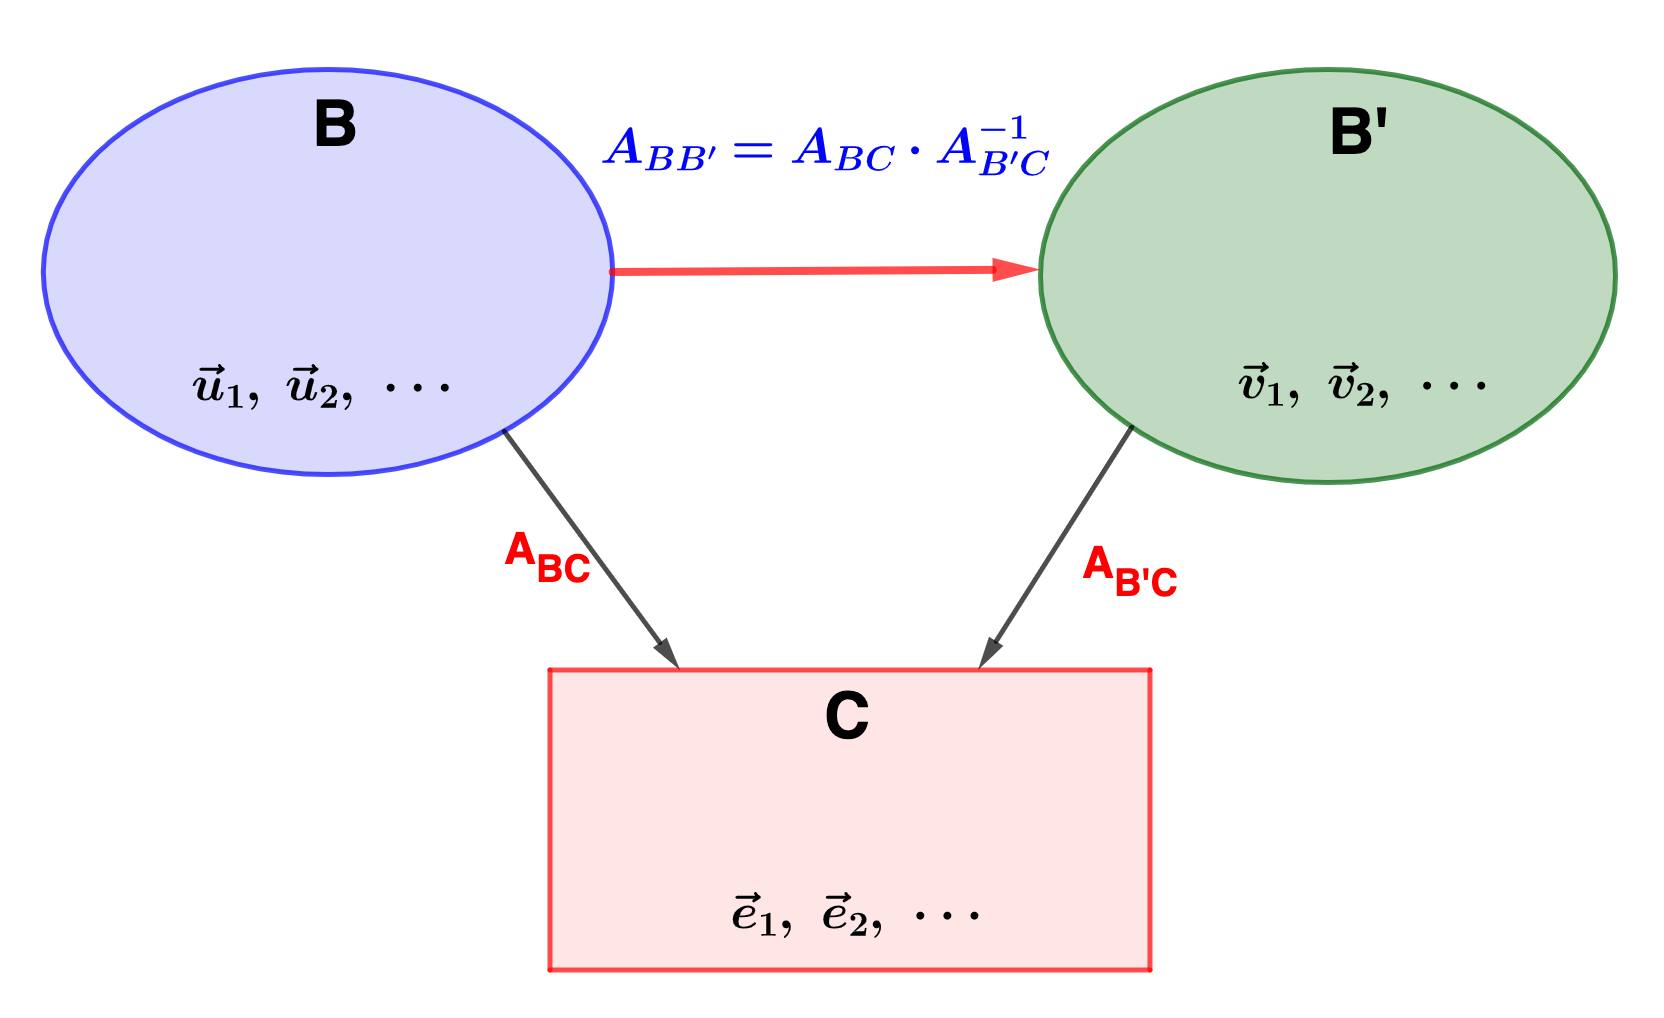
\includegraphics[width=0.7\textwidth]{imagenes/imagenes06/T06IM01.png}
		\caption*{Matriz de cambio de base.}
\end{figure}


\begin{myexampleblock}{Historia de los espacios vectoriales}

La noción de espacio vectorial se utiliza para nombrar a la estructura matemática que se crea a partir de un conjunto no vacío y que cumple con diversos requisitos y propiedades iniciales. Esta estructura surge mediante una operación de suma (interna al conjunto) y una operación de producto entre dicho conjunto y un cuerpo.

\vspace{2mm} Es importante tener en cuenta que todo espacio vectorial dispone de una base y que todas las bases de un espacio vectorial, a su vez, presentan la misma cardinalidad.

\vspace{2mm} \underline{Datos históricos y aplicaciones}:

\vspace{2mm} Fue a partir del siglo XVII que los estudiosos comenzaron a caminar hacia la concepción de los espacios vectoriales, con temas tales como las matrices, los sistemas de ecuaciones lineales y la geometría analítica (al introducir coordenadas en el espacio tridimensional -3D- o el plano -2D-).

\vspace{2mm} Cerca del año 1636, Descartes y Fermat (célebres científicos originarios de Francia) establecieron los fundamentos de la geometría analítica, tomando una ecuación con dos variables y vinculando sus soluciones con la determinación de una curva plana. Para conseguir una solución dentro de los límites de la geometría sin necesidad de recurrir a las coordenadas, el matemático checo Bernard Bolzano presentó un siglo y medio más tarde algunas operaciones sobre planos, líneas y puntos que pueden considerarse antecesores de los vectores.

\vspace{2mm} Sin embargo, recién a finales del siglo XIX, Giuseppe Peano, conocido matemático italiano, realizó la primera formulación moderna y axiomática de los espacios vectoriales. 

\vspace{2mm} Cabe mencionar que los vectores como concepto propiamente dicho nacen con el `bipoint’ de Giusto Bellavitis, un segmento orientado que posee un extremo llamado origen y otro, extremo. Más tarde, fue tomado en cuenta cuando Argand y Hamilton presentaron los números complejos y este último creó los cuaterniones, además de ser quien concibió la denominación de vector. Laguerre, por su parte, fue responsable de la definición de los sistemas de ecuaciones lineales y de la combinación lineal de vectores.

\vspace{2mm} Entre las aplicaciones de los espacios vectoriales se encuentran ciertas funciones de compresión de sonido e imágenes, que se basan en las series de Fourier y otros métodos, y la resolución de ecuaciones en derivadas parciales (relacionar una función matemática con diversas variables independientes y las derivadas parciales de la misma respecto de dichas variables). Por otro lado, sirven para el tratamiento de objetos físicos y geométricos, como son los tensores.

\vspace{6mm} \emph{Cuando en varios conjuntos distintos aparecen estructuras similares, es conveniente axiomatizar éstas y dar un nombre al ente resultante. Aunque esto tiene el inconveniente de trabajar en el mundo abstracto de los espacios vectoriales arbitrarios, también presenta una gran ventaja}.


\vspace{2mm} \emph{ La abstracción resulta ser matemáticamente eficiente en el sentido de que ahora pueden demostrarse resultados generales cuya validez afecta a todos los espacios vectoriales. Es decir, una vez que se establecen los hechos sobre los espacios vectoriales en general, se pueden aplicar estos hechos a todos los espacios vectoriales. De otro modo, habría que probar cada hecho una y otra vez, para cada nuevo espacio vectorial que nos encontráramos (y existen un sin fin de ellos).}
	
\end{myexampleblock}




	%\begin{figure}[H]
		%\centering
		%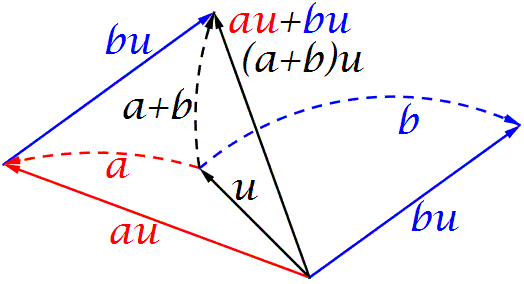
\includegraphics[width=0.5\textwidth]{imagenes/imagenes01/T01IM01.png}
		%\caption{Los dos problemas clásicos del cálculo: trazado de tangentes y áreas bajo curvas.}
	%\end{figure}
		
%varios párrafos encuadrados - explicaciones ad hoc
%\centering{
%\fbox{
%\parbox{0.95\textwidth}{
%varios
%
%$parrafos
%
%dentro
%}
%}
%}
% \justify


%\rotatebox{180}{\leftline{\textcolor{gris}{tararí}}}.